\documentclass[9pt, aspectratio=169]{beamer}
\usepackage{FiraSans}
\usetheme[subsectionpage=progressbar]{metropolis}
\usepackage[utf8]{inputenc}
\usepackage{amsmath}
\usepackage{amsfonts}
\usepackage{amssymb}
\usepackage{multicol}
\usepackage{tikz}
\usetikzlibrary{matrix}
\usepackage{xcolor}
\usepackage{subcaption}
\usepackage[T1]{fontenc} 
\usepackage[skins]{tcolorbox}
\author{Nicola Roman\`o - nicola.romano@ed.ac.uk}
\title{Lecture 6 - Image features}
\setlength{\fboxsep}{0pt}
% Remove "Figure" in front of captions
% See https://tex.stackexchange.com/questions/82456/how-to-remove-figure-caption-prefix-figure-in-beamer
\captionsetup{labelformat=empty,labelsep=none}
\setbeamertemplate {footline}{\begin{scriptsize}\hfill\insertframenumber ~of \inserttotalframenumber\kern1em\vskip5pt\end{scriptsize}}

\titlegraphic{\centering 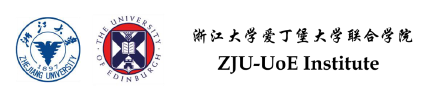
\includegraphics[scale=.5]{instituteLogo.png}}
\date{}

\begin{document}

\newtcolorbox{codebox}{enhanced,
    top=2pt,
    left=2pt,
    right=2pt,
    bottom=2pt,
    boxrule=0pt,
    leftrule=5pt,
    sharp corners,
    colback=gray!20,
    colframe=blue!60!black}

\begin{frame}
    \titlepage
\end{frame}

\begin{frame}
    {Learning objectives}
    \begin{columns}
        \begin{column}{0.8\textwidth}
            \begin{itemize}
                \item Define and give examples of image features
                \item Describe and apply methods to extract geometric features in an image
                \item Describe and apply methods for texture analysis in images
                \item Discuss advantages and issues with these methods
            \end{itemize}
        \end{column}
        \begin{column}{0.2\textwidth}
            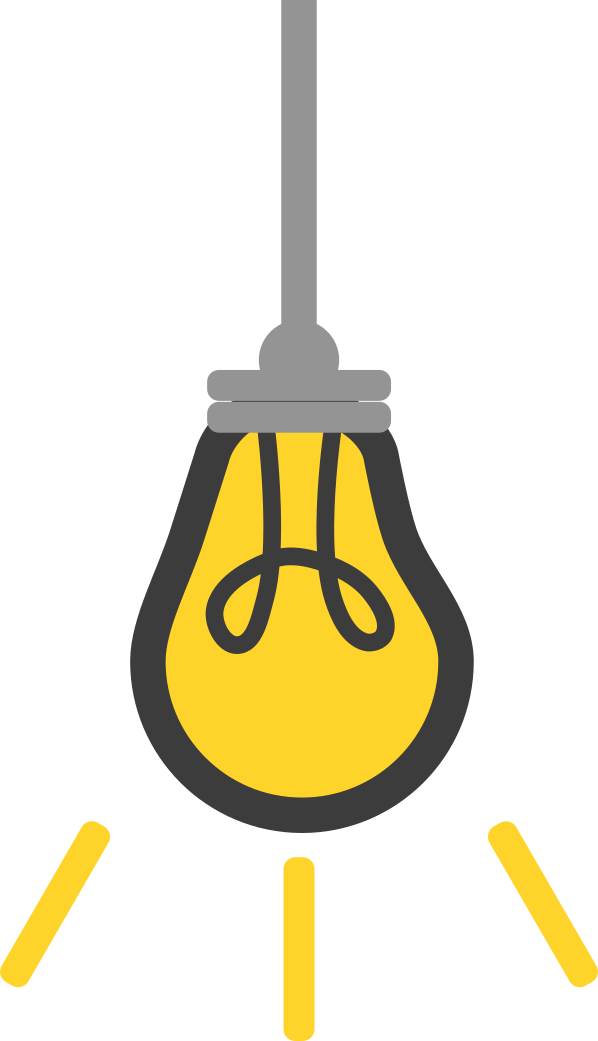
\includegraphics[angle=-30, origin=tr, width=1.5\textwidth]{lightbulb.png}
        \end{column}
    \end{columns}
\end{frame}

\section{What is a feature?}

\begin{frame}
    {Features}
    \textbf{Feature}, n.: a distinctive or characteristic part of a thing; some part which arrests the attention by its conspicuousness or prominence.\\
    (\textit{Source: Oxford English Dictionary})
    \pause

    \vspace{2em}

    In image analysis, a \textbf{feature} is a characteristic of the image, or of a part of it, that defines some of its properties.

    Examples of features include edges, corners, ridges, texture, colour, shape etc.

    \pause
    \vspace{2em}
    Detecting features is a fundamental step to extract information from images.
\end{frame}

\begin{frame}
    {Features in images}
    \begin{figure}
        \includegraphics[width=\textwidth]{mountain.jpg}
        \caption{\small{\color{gray}{View in the Gran Sasso mountain range, Italy - Photo: Nicola Roman\`o}\color{black}}}
    \end{figure}
    \centering
    \textbf{Which are the prominent features of this image?}
\end{frame}

\begin{frame}
{Why detect features?}
Examples of tasks for which we may use features
\begin{itemize}[<+->]
\item To detect whether specific objects are present in an image and where
\item To track the position of objects in an video (by using the position of specific features)
\item To classify images (by using features as descriptors)
\item To stitch images together
\end {itemize}

\centering
\only<1>
{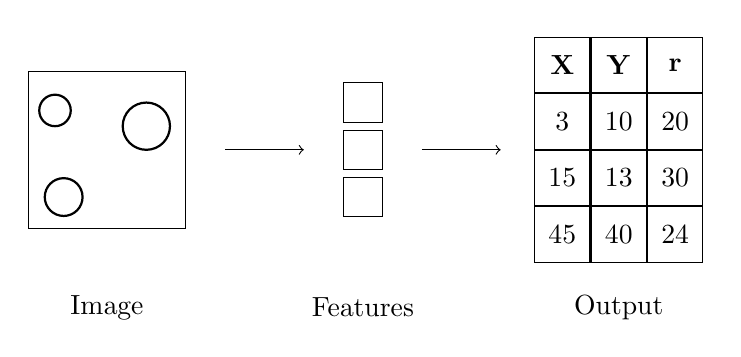
\begin{tikzpicture}
        \draw (0, 0) rectangle (2, 2);
        \draw [thick](0.34,1.5) circle (.2);
        \draw [thick](1.5, 1.3) circle (.3);
        \draw [thick](0.45, 0.4) circle (.24);
        \node at (1, -1) {Image};
        \draw [->] (2.5, 1) -- (3.5, 1);
        \foreach \i in {0.25,...,2.25}
            {
                \draw (4, \i * .6) rectangle (4.5, \i * .6 + .5);
            }
        \node at (4.25, -1) {Features};
        \draw [->] (5, 1) -- (6, 1);
        \matrix[matrix of nodes,nodes={draw},ampersand replacement=\&, minimum height=2em, minimum width=2em, nodes={anchor=center}] at (7.5, 1) {
            \textbf{X} \& \textbf{Y} \& \textbf{r} \\
            3 \& 10 \& 20                                                              \\
            15 \& 13 \& 30                                                             \\
            45 \& 40 \& 24                                                             \\
        };
        \node at (7.5, -1) {Output};
    \end{tikzpicture}
}

\only<2>{
    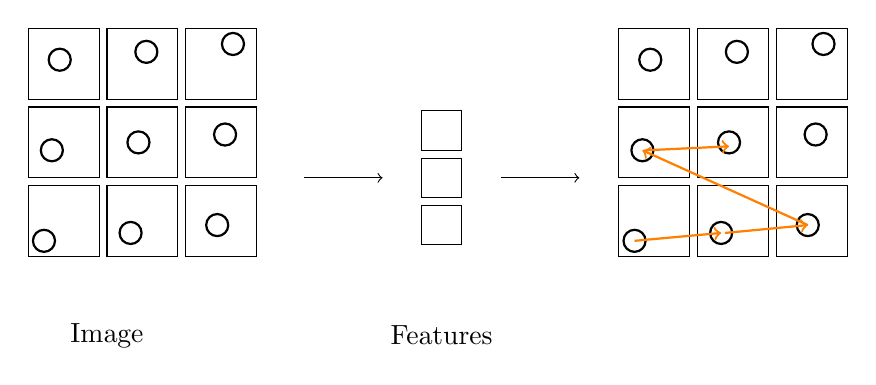
\begin{tikzpicture}
        \foreach \x in {0, 1, 2}
            {
                \foreach \y in {0, 1, 2}
                    {
                        \draw (\x, \y) rectangle (\x + 0.9, \y + 0.9);
                        \draw [thick](\x + .2 + .1 * \x + .1 * \y, \y + .2 + .1 * \x + .15 * \y) circle (.14);
                    }
            }
        \node at (1, -1) {Image};
        \draw [->] (3.5, 1) -- (4.5, 1);
        \foreach \i in {0.25,...,2.25}
            {
                \draw (5, \i * .6) rectangle (5.5, \i * .6 + .5);
            }
        \node at (5.25, -1) {Features};

        \draw [->] (6, 1) -- (7, 1);

        \foreach \x in {7.5, 8.5, 9.5}
            {
                \foreach \y in {0, 1, 2}
                    {
                        \draw (\x, \y) rectangle (\x + 0.9, \y + 0.9);
                        \draw [thick] (\x - .55 + .1 * \x + .1 * \y, \y + -0.55 + .1 * \x + .15 * \y) circle (.14);
                    }
            }

        \draw [->, color=orange, thick] (7.7, 0.2) -- (8.8, 0.3);
        \draw [->, color=orange, thick] (8.85, 0.3) -- (9.9, 0.4);
        \draw [->, color=orange, thick] (9.9, 0.4) -- (7.8, 1.35);
        \draw [->, color=orange, thick] (7.85, 1.35) -- (8.9, 1.4);
    \end{tikzpicture}
}

\only<3>{
    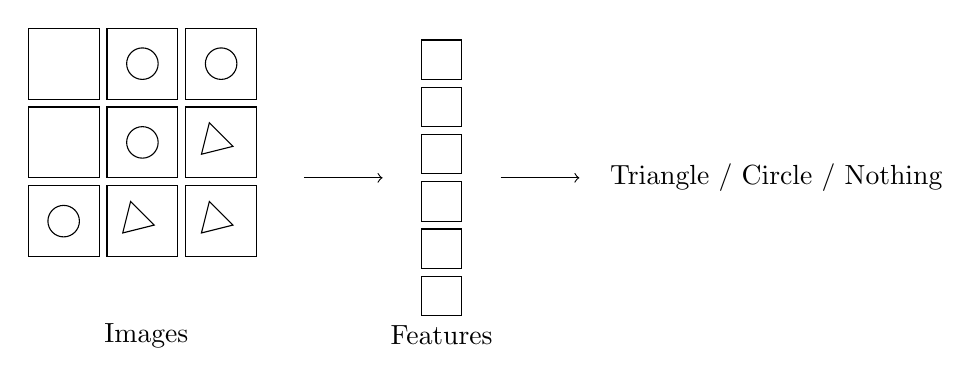
\begin{tikzpicture}
        \foreach \x in {0, 1, 2}
            {
                \foreach \y in {0, 1, 2}
                    {
                        \draw (\x, \y) rectangle (\x + 0.9, \y + 0.9);
                    }
            }

        \draw (0.45, 0.45) circle (.2);
        \draw (1.45, 2.45) circle (.2);
        \draw (1.45, 1.45) circle (.2);
        \draw (2.45, 2.45) circle (.2);
        \draw (1.2, 0.3) -- (1.6, 0.4) -- (1.3, 0.7) -- cycle;
        \draw (2.2, 0.3) -- (2.6, 0.4) -- (2.3, 0.7) -- cycle;
        \draw (2.2, 1.3) -- (2.6, 1.4) -- (2.3, 1.7) -- cycle;

        \node at (1.5, -1) {Images};
        \draw [->] (3.5, 1) -- (4.5, 1);
        \foreach \i in {-1.25,...,4.25}
            {
                \draw (5, \i * .6) rectangle (5.5, \i * .6 + .5);
            }
        \node at (5.25, -1) {Features};

        \draw [->] (6, 1) -- (7, 1);

        \node at (9.5, 1) {Triangle / Circle / Nothing};
    \end{tikzpicture}
}

\only<4>{
    \begin{tikzpicture}
        \draw (0, 0) rectangle (2, 2);
        \draw (2.5, 0) rectangle (4.5, 2);
        \draw (1, 1) circle (0.5);
        \draw (1.5, 1.5) rectangle(2, 1.8);
        \draw (1.9, 0.2) rectangle(2, 0.4);

        \draw (2.5, 1.5) rectangle(2.8, 1.8);
        \draw (2.5, 0.2) rectangle(3.5, 0.4);

        \node at (2.25, -1) {Images};

        \draw [->] (5, 1) -- (6, 1);
        \foreach \i in {-1.25,...,4.25}
            {
                \draw (6.5, \i * .6) rectangle (7, \i * .6 + .5);
            }
        \node at (6.75, -1) {Features};

        \draw [->] (7.5, 1) -- (8.5, 1);

        \draw (9, 0) rectangle (13, 2);

        \draw (10, 1) circle (0.5);
        \draw (10.5, 1.5) rectangle(11.3, 1.8);
        \draw (10.9, 0.2) rectangle(12, 0.4);
    \end{tikzpicture}
}
\end{frame}

\section{Geometric features}

\begin{frame}
    {Geometric features}
    \centering
    Examples of \textbf{geometric features} include:\\
    \vspace{2em}

    \begin{figure}
        \centering
        \subcaptionbox{\centering \textbf{Blobs} - \color{gray}{Marsh et al., Sci Rep 2018}}
        {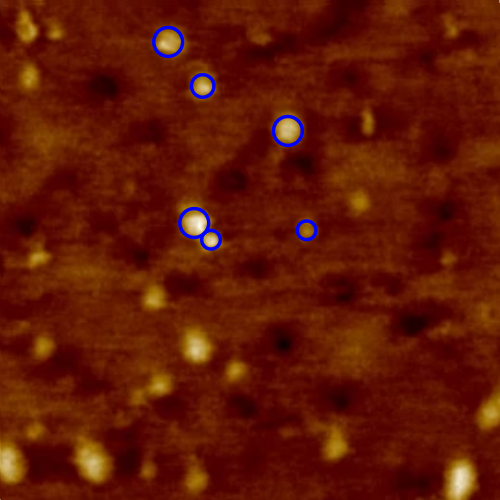
\includegraphics[width=.22\textwidth]{AFM - Marsh 2018.png}}
        \subcaptionbox{\centering \textbf{Corner and edges} (see lecture 5) - \color{gray}{Credits: Masur, Wikipedia, CC-0}}
        {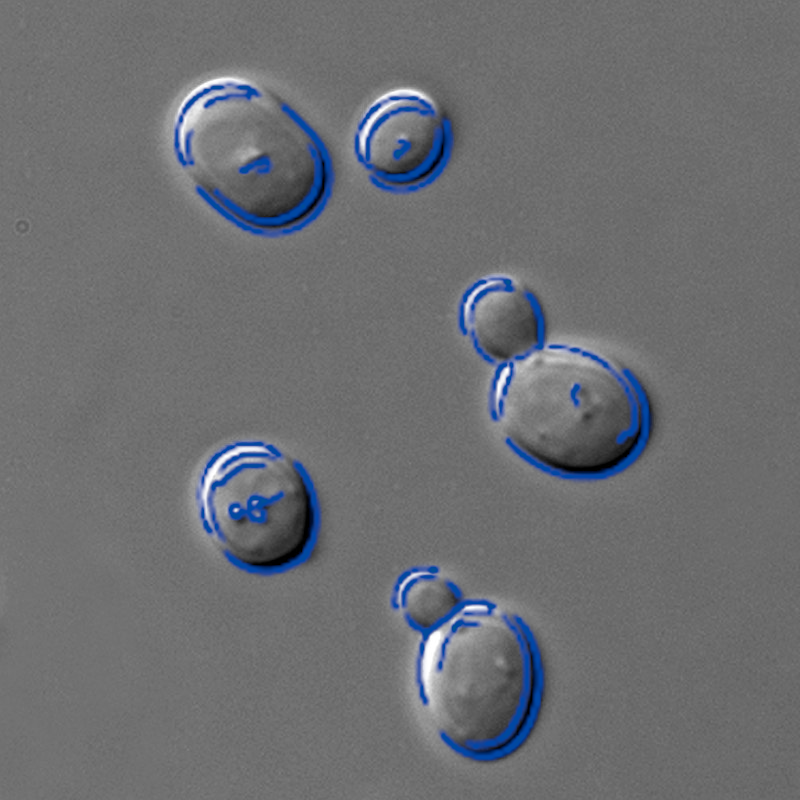
\includegraphics[width=.22\textwidth]{yeast.png}}
        \subcaptionbox{\centering \textbf{Lines, circles, etc.} - \color{gray}{Credits: Vivien Rolfe, Flickr, CC-BY-SA-2.0}}
        {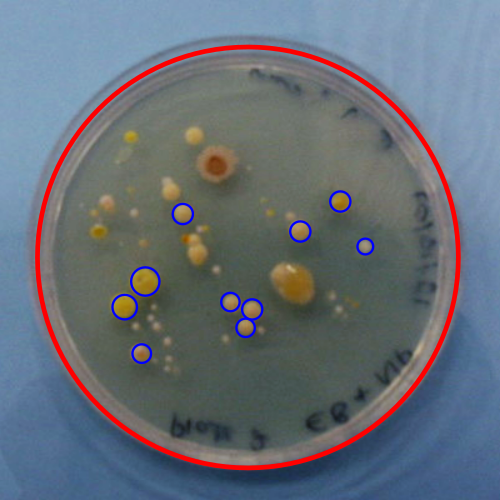
\includegraphics[width=.22\textwidth]{plate.png}
        }
        \subcaptionbox{\centering \textbf{Ridges} - \color{gray}{Credits:  Medical gallery of Mikael H\"aggstr\"om., CC-0}}
        {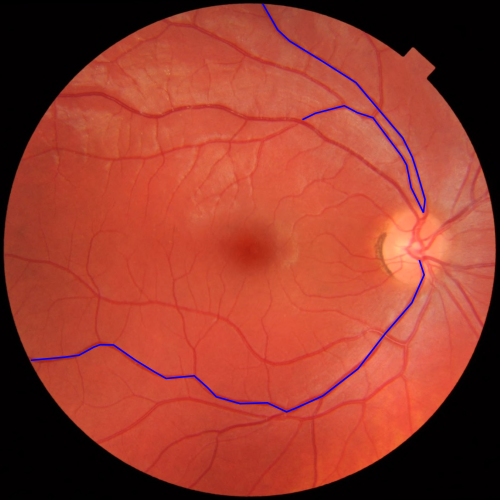
\includegraphics[width=.22\textwidth]{retina_vessels.png}}
    \end{figure}
\end{frame}

\subsection{Blobs}

\begin{frame}
    {Blob detection}
    Blob detection is the task of detecting blobs in an image.

    \textbf{Blobs} are defined as regions of pixels with uniform properties that are clearly distinguishable from the background.

    There are many methods for detecting blobs in an image; today we will look at using the Laplacian of the Gaussian (\textbf{LoG}) method, and its approximation by the difference of Gaussians (\textbf{DoG}) method.
\end{frame}

\begin{frame}
    {The Laplacian operator}
    In the last lecture we talked about using second order derivatives to detect edges in an image.
    The Laplacian of Gaussian operator is defined as the sum of the second order partial derivatives of the image.
    \large{
    $$\text{Laplacian(I)} = \nabla^2(I) = \frac{\partial^2{I}}{\partial{x^2}} + \frac{\partial^2{I}}{\partial{y^2}}$$
    }
\end{frame}

\begin{frame}
    {The Laplacian of the Gaussian}
    \centering
    What does the Laplacian of a Gaussian function look like?

    \begin{figure}
        \centering
        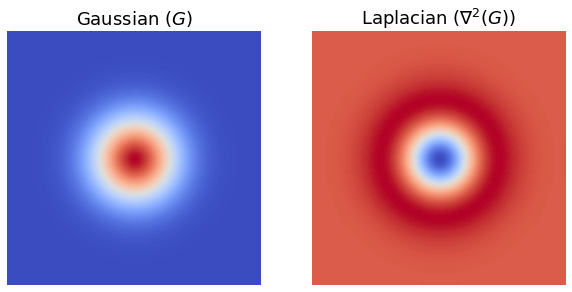
\includegraphics[width=.45\textwidth]{gaussian_and_laplacian_2D.png}
        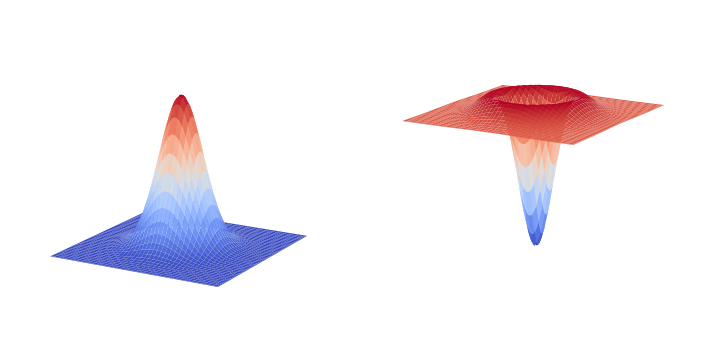
\includegraphics[width=.45\textwidth]{gaussian_and_laplacian_3D.png}
    \end{figure}
    \centering
    So... how do we use this to detect blobs?
\end{frame}

\begin{frame}
    {The LoG method for blob detection}
    The idea is to:

    \begin{enumerate}
        \item Apply a LoG filter $LoG(\sigma)$ to the image, as discussed in Lecture 5
        \item Dark blobs on light background will appear as bright spots in the Laplacian of the Gaussian-filtered image; bright blobs on dark background will appear as dark spots.
              \pause
        \item We find local maxima (or minima) in the Laplacian of the Gaussian-filtered image to determine the position of the blobs
        \item The blob size is approximately $\sqrt{2}\sigma$ (or $\sqrt{3}\sigma$ for 3D)
    \end{enumerate}
\end{frame}

\begin{frame}
    {The DoG method for blob detection}
    \only<1->{To detect blobs of different size, we can use a Gaussian filter with different standard deviations.}

    \pause
    \only<2>{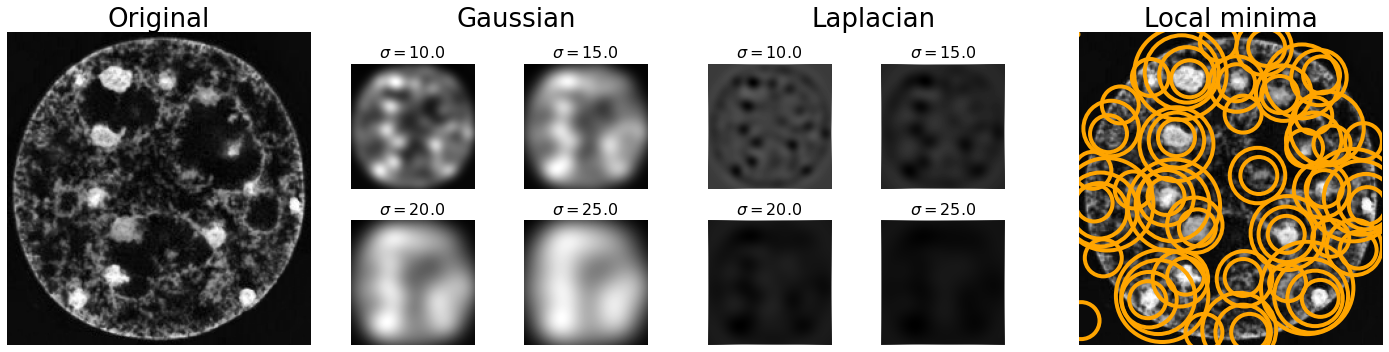
\includegraphics[width=\textwidth]{blob_detection_thr0.png}}
    \only<3>{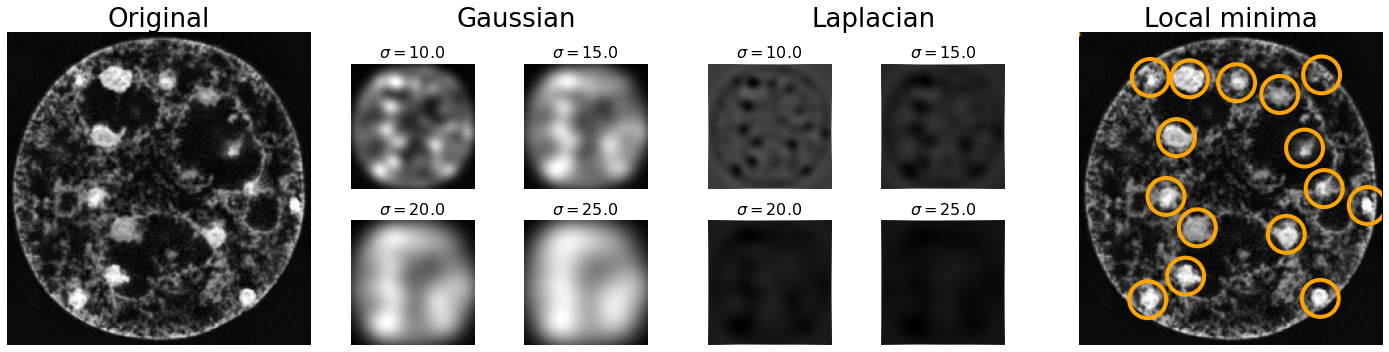
\includegraphics[width=\textwidth]{blob_detection_thr0_4.png}}
    \only<4->{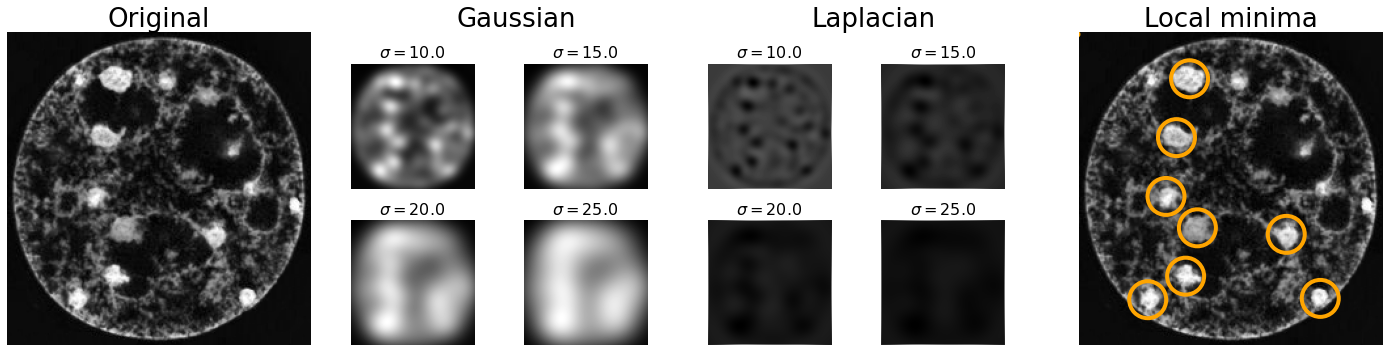
\includegraphics[width=\textwidth]{blob_detection_thr0_8.png}}

    \only<2->{We can apply a threshold to the DoG image to remove spurious blobs and can also remove blobs overlapping over a certain \%}

    \only<5>{Scikit image implements these steps in the \href{https://scikit-image.org/docs/dev/api/skimage.feature.html\#skimage.feature.blob\_log}{\texttt{skimage.feature.blob\_log}} function.}
\end{frame}

\begin{frame}
    {Example of blob detection}
    \begin{columns}
        \begin{column}{.7\textwidth}
            \begin{codebox}
                \texttt{from skimage.feature import blob\_log\\
                    from skimage.io import imread\\
                    \\
                    nucleus = imread("nucleus\_blob.png")\\
                    blobs = blob\_log(nucleus, min\_sigma=10, max\_sigma=15,
                    $~~~~~~~~~~~~~~~~~$num\_sigma=5, threshold=0.3, overlap=.4)\\
                    \pause
                    plt.imshow(nucleus, cmap="gray")\\
                    \\
                    for b in blobs:\\
                    $~~~~$y, x, radius = b\\
                    $~~~~$\# Create a circle at the blob center\\
                    $~~~~$c = plt.Circle((x, y), radius, color='orange',
                    $~~~~~~~~~~~~~~~~~~~$linewidth=3, fill=False)\\
                    $~~~~$\# Draw the circle (gca = "get current axis")\\
                    $~~~~$plt.gca().add\_artist(c)\\
                    plt.show()
                }
            \end{codebox}
        \end{column}
        \begin{column}{.3\textwidth}
            \only<2>{
                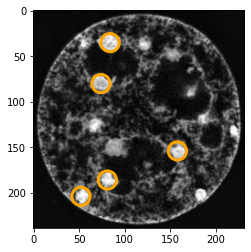
\includegraphics[width=\textwidth]{blob_log_example.png}
            }
        \end{column}
    \end{columns}
\end{frame}

\begin{frame}
    {Other methods for blob detection}
    Scikit image impements two other methods for blob detection: the DoG (Difference of Gaussians) and the DoH (Determinant of the Hessian) methods.

    \pause

    The \textbf{DoG method} is a fast approximation of the LoG method. It works by calculating the difference between two version of the image blurred by Gaussians with different $\sigma$.

    The \textbf{DoH method} is the fastest method. It works by calculating the determinant of the Hessian of the image (the \href{https://en.wikipedia.org/wiki/Hessian\_matrix}{\underline{Hessian}} is a matrix of second partial derivatives).
    Contrary to DoG and LoG, the detection speed is independent of the size of the blobs. However, DoH is less accurate at detecting small blobs.

    \pause
    These are implemented in \href{https://scikit-image.org/docs/dev/api/skimage.feature.html\#skimage.feature.blob\_dog}{\texttt{\underline{skimage.feature.blob\_dog}}} and \href{https://scikit-image.org/docs/dev/api/skimage.feature.html\#skimage.feature.blob\_doh}{\texttt{\underline{skimage.feature.blob\_doh}}} respectively.
\end{frame}

\subsection{Lines and circles (the Hough transform)}

\begin{frame}
    {The Hough transform}
    The Hough transform is a technique originally developed by Paul Hough in 1962 for finding straight lines in an image. Extensions of this technique allow to find circles and quadrilaterals.
    \centering
    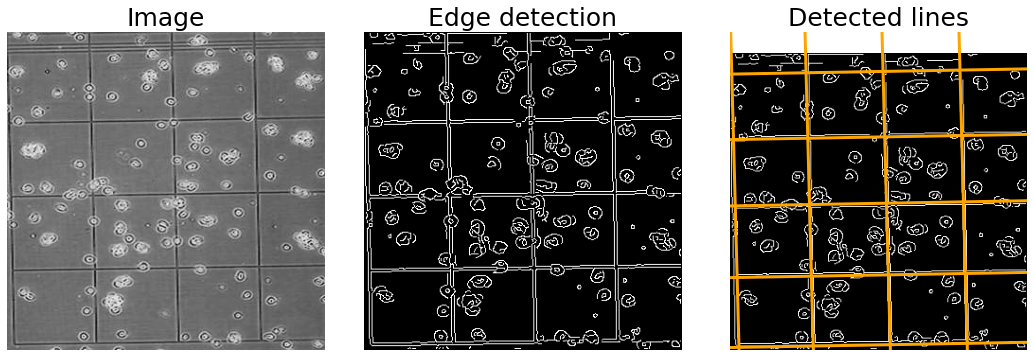
\includegraphics[width=.85\textwidth]{hough_line_overview.png}
\end{frame}

\begin{frame}
    {Representing a line}
    \begin{columns}
        \begin{column}{.5\textwidth}
            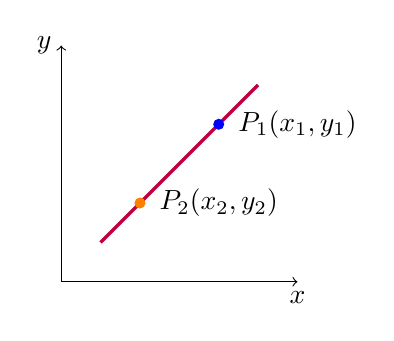
\begin{tikzpicture}
                \draw[thin,->] (0,0) -- (3,0) node[below] {$x$};
                \draw[thin,->] (0,0) -- (0,3) node[left] {$y$};
                \draw[purple, very thick] (0.5, 0.5) -- (2.5, 2.5);
                \fill [orange] (1, 1) circle (2pt);
                \fill [blue] (2, 2) circle (2pt);
                \node at (3, 2) {$P_1(x_1, y_1$)};
                \node at (2, 1) {$P_2(x_2, y_2$)};
            \end{tikzpicture}

            Consider a line with equation: $y = a\cdot x + b$ and two points $P_1$ and $P_2$ on it.
        \end{column}
        \pause
        \begin{column}{.5\textwidth}
            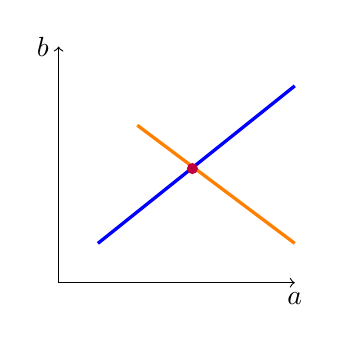
\begin{tikzpicture}
                \draw[thin,->] (0,0) -- (3,0) node[below] {$a$};
                \draw[thin,->] (0,0) -- (0,3) node[left] {$b$};
                \draw [orange, very thick] (1, 2) -- (3, 0.5);
                \draw [blue, very thick] (0.5, 0.5) -- (3, 2.5);
                \fill [purple] (1.7, 1.45) circle (2pt);
                % \fill [blue] (2, 1) circle (2pt);
                % \node at (2, 2) {($x_1, y_1$)};
                % \node at (3, 1) {($x_2, y_2$)};
            \end{tikzpicture}

            The families of lines passing through $P_1$ (or $P_2$) have equation: $b = - x_1\cdot a + y_1$ (or $b = - x_2\cdot a + y_2$).
            \pause
        \end{column}
    \end{columns}

    The intersection is the slope and intercept of the original line! Any point on the red line on the left will correspond to a line passing through the red point in the $a/b$ space.\\
    \textbf{This is the principle of the Hough transform.}
\end{frame}

\begin{frame}
    {Representing a line - another way}
    We can also represent a line in terms of an angle and a distance from the origin. This is a better alternative, because we can also use it to represent a vertical line.\\

    \large
    \begin{center}
        $x \cdot \cos(\theta) + y \cdot \sin(\theta) = \rho$
    \end{center}

    \begin{columns}
        \begin{column}{.5\textwidth}
            \normalsize
            Where $\theta$ is the angle of the line and $rho$ is the distance from the origin.

            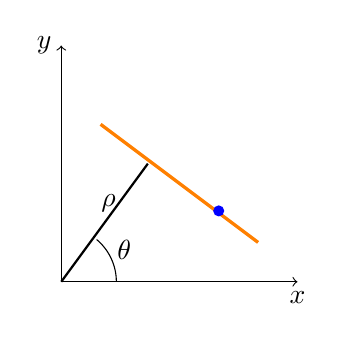
\begin{tikzpicture}
                \draw[thin,->] (0,0) -- (3,0) node[below] {$x$};
                \draw[thin,->] (0,0) -- (0,3) node[left] {$y$};
                \draw [thick] (0, 0) -- (1.1, 1.5);
                \draw [orange, very thick] (0.5, 2) -- (2.5, 0.5);
                \draw (0.7, 0) arc (0:50:.7) node at (.8, .4) {$\theta$}
                ;
                \node at (.6, 1) {$\rho$};
                \fill [blue] (2, 0.9) circle (2pt);
            \end{tikzpicture}
        \end{column}
        \pause
        \begin{column}{.5\textwidth}
            \normalsize
            We can map each point in the $\theta/\rho$ space (called the Hough space) as we did before.

            \begin{tikzpicture}
                \draw[thin,->] (0,0) -- (3,0) node[right] {$\theta$};
                \draw[thin,->] (1.4,0) -- (1.4,3) node[left] {$\rho$};
                \node at (0, -.2) {$-\pi$};
                \node at (2.8, -.2) {$\pi$};
                \draw [blue] plot [smooth, tension=1.2] coordinates { (0,2.4) (0.5, 2.2) (1,1.6) (2,0.5) (2.9,0.7)};
            \end{tikzpicture}
        \end{column}
    \end{columns}
\end{frame}

\begin{frame}
    {The Hough transform}
    There are three steps in the Hough transform:

    \begin{enumerate}[<+->]
        \item Edge detection - e.g. using the Canny edge detector. This gives us a binary image.
        \item We create a $M x N$ matrix of 0s, representing the Hough space. This will correspond to $M$ different values of $\rho$ and $N$ different values of $\theta$.
        \item Iterate through all the pixels of the image and if they are an edge map they get to "cast a vote" onto the Hough space.
        \item Each value in the Hough space matrix is use as an "accumulator". We add 1 to the value of the Hough space at the corresponding $\theta$ and $\rho$ coordinates for each possible line passing through the edge point.
        \item The Hough space matrix is then thresholded and non-maximum-suppression applied to find the strongest lines.
    \end{enumerate}
\end{frame}

\begin{frame}
    {Hough transform - an example}
    \only<1>{
        \begin{codebox}
            \texttt{from skimage.feature import canny\\
                from skimage.transform import hough\_line, hough\_line\_peaks\\
                \\
                chamber = imread("cell\_counting\_chamber.jpg")\\
                chamber\_canny = canny(chamber, sigma=1.5)}
        \end{codebox}
        \centering
        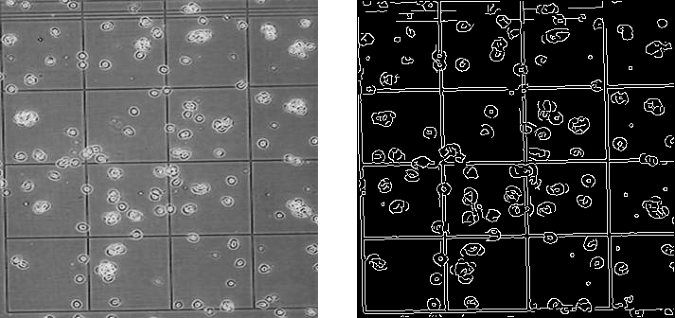
\includegraphics[width=.6\textwidth]{chamber_and_canny.png}
    }
    \only<2>{
        \begin{codebox}
            \texttt{hough\_space, angles, d = hough\_line(chamber\_canny)\\
            accum, theta, rho = hough\_line\_peaks(hough\_space, angles, d)\\
            for t, r in zip(theta, rho):\\
            $~~~~$print(f"{np.rad2deg(t):0.2f}, {r:0.2f}")
            }
        \end{codebox}
        \begin{columns}
            \begin{column}{.7\textwidth}
                \centering
                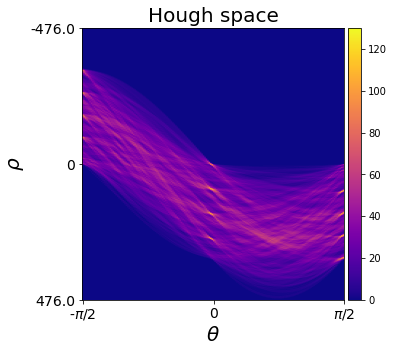
\includegraphics[width=.7\textwidth]{chamber_hough_space.png}
            \end{column}
            \begin{column}{.23\textwidth}
                \begin{codebox}
                    \texttt{88.99, 253.77\\
                        88.99, 97.60\\
                        -1.51, 258.77\\
                        -1.51, 171.68\\
                        88.99, 332.85\\
                        -1.51, 84.59\\
                        88.99, 172.68\\
                        -1.51, 0.50\\
                        88.99, 23.52
                    }
                \end{codebox}
            \end{column}
        \end{columns}

    }
\end{frame}

\begin{frame}
    {The circle Hough transform}
    \begin{columns}
        \begin{column}{.6\textwidth}
            It is easy to extend the Hough transform to circles.

            A circle with radius $r$ and centre $(a; b)$ has equation

            $$(x - a)^2 + (y - b)^2 = r^2$$

            \pause
            We can create a 3D Hough space $(a, b, r)$ and proceed as before, testing a number of different radii.

            \only<3->{The circle Hough transform is implemented in the \texttt{hough\_circle} and \texttt{hough\_circle\_peaks} functions.

                \vspace{1em}

                \small
                \textit{On the right}: example of the circle Hough transform (top detected circles, bottom the Hough space for the larger radius). Note the spurious detection of a small circle at the top left of the image. - Source: Kwak et al, 2009}
        \end{column}
        \begin{column}{.4\textwidth}
            \only<3->
            {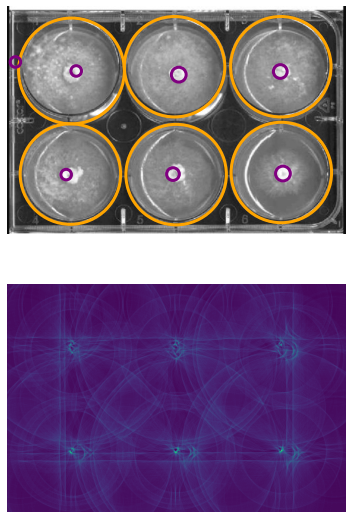
\includegraphics[width=.9\textwidth]{hough_circle.png}}
        \end{column}
    \end{columns}
\end{frame}

\section{Texture features}

\begin{frame}
    {Texture features}
    Texture features describe the local appearance of an image.\\

    The texture of an image is determined by the spatial distribution of intensity levels in a neighborhood.

    Given the neighborhood of a pixel, we can define basic texture features such as:

    \begin{enumerate}
        \item \textbf{Range}: max intensity - min intensity
        \item \textbf{Variance}: variance of the intensity values in the neighborhood
    \end{enumerate}
    \pause

    \centering
    \begin{figure}
        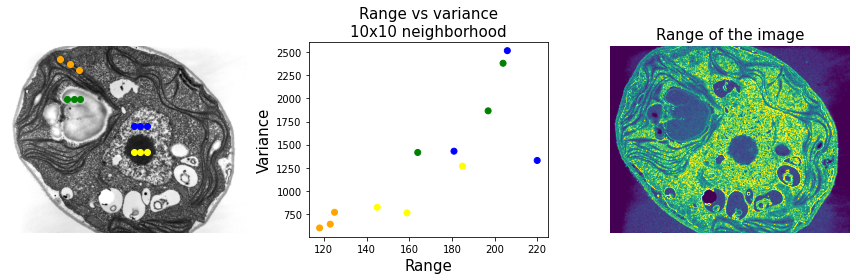
\includegraphics[width=.8\textwidth]{texture_features_range_var.png}
        \caption{\small{\color{gray}{TEM image of a Chlamydomonas green algae - CC0, Dartmouth College}\color{black}}}
    \end{figure}
\end{frame}

\begin{frame}
    {Entropy}
    In information theory, \textbf{entropy} is a quantity related to the complexity of information in a system.

    For an image, entropy is the minimum number of bits needed to encode the local greylevel distribution.

    Entropy can be calculated using the \href{https://scikit-image.org/docs/dev/api/skimage.filters.rank.html\#skimage.filters.rank.entropy}{\texttt{\underline{skimage.filters.rank.entropy}}} function.

    \begin{codebox}
        \texttt{from skimage.filters.rank import entropy\\
            im\_entr = entropy(image, selem=np.ones((5, 5))}
    \end{codebox}
    \centering
    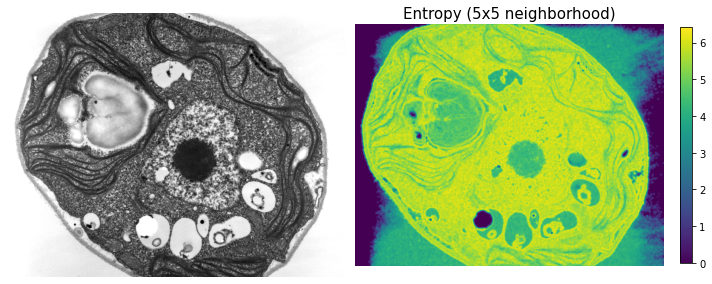
\includegraphics[width=.75\textwidth]{entropy.png}
\end{frame}

\begin{frame}
    {GLCM features}
    A more quantitative approach to texture features is the \textbf{grey-level co-occurrence matrix (GLCM)}.\\
    \vspace{2em}

    A GLCM is definted as a $n\times n$ matrix of values counting the pixels with a specific intensity at a certain distance and angle in the image. $n$ is the number of grey levels in the image.\\
\end{frame}

\begin{frame}
    {Example GLCM}
    \begin{columns}
        \begin{column}{.5\textwidth}
            \centering
            \textbf{Image}\\

            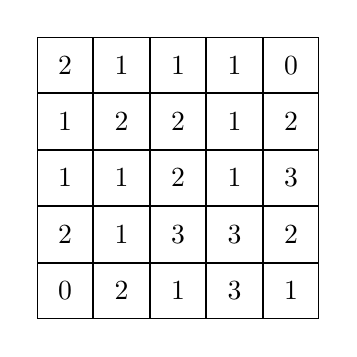
\begin{tikzpicture}
                \matrix[matrix of nodes,nodes={draw},ampersand replacement=\&, minimum height=2em, minimum width=2em, nodes={anchor=center}]{
                    2 \& 1 \& 1 \& 1 \& 0 \\
                    1 \& 2 \& 2 \& 1 \& 2 \\
                    1 \& 1 \& 2 \& 1 \& 3 \\
                    2 \& 1 \& 3 \& 3 \& 2 \\
                    0 \& 2 \& 1 \& 3 \& 1 \\
                };
            \end{tikzpicture}
        \end{column}
        \begin{column}{.5\textwidth}
            \centering
            \textbf{GLCM (distance=1, angle=0)}\\

            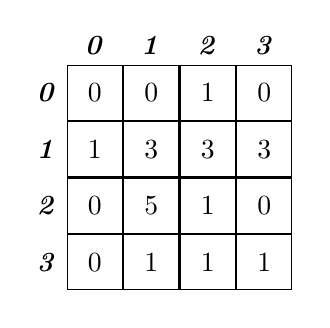
\begin{tikzpicture}
                \matrix (m) [matrix of nodes,nodes={draw},ampersand replacement=\&, minimum height=2em, minimum width=2em, nodes={anchor=center}]{
                    0 \& 0 \& 1 \& 0 \\
                    1 \& 3 \& 3 \& 3 \\
                    0 \& 5 \& 1 \& 0 \\
                    0 \& 1 \& 1 \& 1 \\
                };
                \foreach \i [count=\xi from 0] in  {1,...,4}{
                        \node also [label=above:\textit{\textbf{\xi}}] (m-1-\i) {};
                        \node also [label=left:\textit{\textbf{\xi}}] (m-\i-1) {};
                    }
            \end{tikzpicture}
        \end{column}
    \end{columns}

    For example, the GLCM above shows that there are five pixels with intensity 2 and 1 at distance 1 and angle 0 (so to the right).
\end{frame}

\begin{frame}
    {What to do with a GLCM?}
    The GLCM itself is not very useful for our purposes, but we can calculate numeric features from it.\\

    After normalising the GLCM to a sum of 1, we can calculate:

    \begin{itemize}
        \item \textbf{Contrast} - a measure of the contrast between each pixel and its neighbor. \Large $\sum_{i,j=0}^{levels-1}P_{i,j}(i-j)^2$
        \item \normalsize \textbf{Dissimilarity} - a measure of distance between each pixel and its neighbor. \Large $\sum_{i,j=0}^{levels-1}P_{i,j}|i-j|$
        \item \normalsize \textbf{Homogeneity} - a measure of the closeness of the distribution of elements in the GLCM - \Large$\sum_{i,j=0}^{levels-1}\frac{P_{i,j}}{1+(i-j)^2}$
        \item \normalsize \textbf{ASM} (angular second moment) -  - \Large $\sum_{i,j=0}^{levels-1}P_{i,j}^2$
        \item \normalsize \textbf{Energy} - $\sqrt{ASM}$
        \item \normalsize \textbf{Correlation} - how correlated neighbour pixels are in an image - \Large $\sum_{i,j=0}^{levels-1}P_{i,j}\frac{(i-\mu_i)(j-\mu_j)}{\sqrt{\sigma_i^2\sigma_j^2}}$
    \end{itemize}

    Again, these are for reference only... don't worry about remembering the formulas!
\end{frame}

\begin{frame}
    {GLCM features - example}
    \centering
    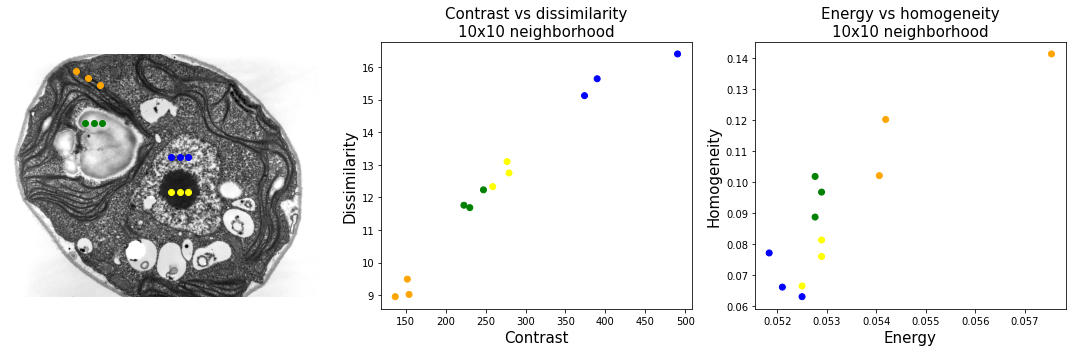
\includegraphics[height=.5\textheight]{glcm_features.png}
    \pause
    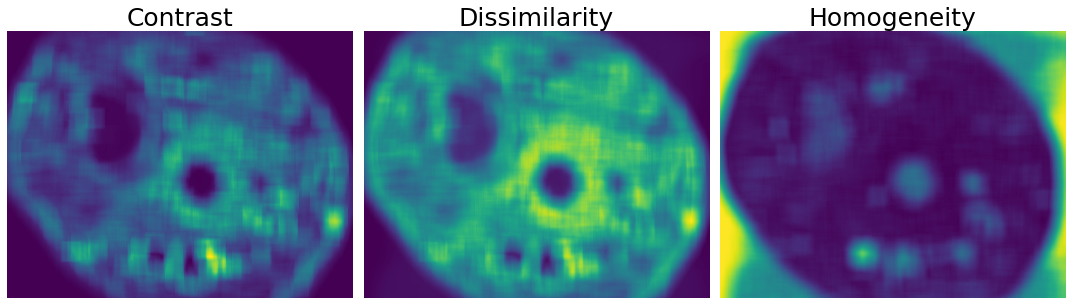
\includegraphics[height=.4\textheight]{glcm_features_b.png}
\end{frame}
\begin{frame}
    {HOG features}
    \textbf{Histogram of oriented gradients (HOG)} features are a set of features that describe the local gradient orientation of an image. They are commonly used for object detection.\\

    \vspace{2em}
    Overview of the algorithm
    \begin{enumerate}[<+->]
        \item \textbf{Global image normalisation} - an optional step to reduce the influence of local changes in illumination. Usually done by computing the log or square root of the image.
        \item \textbf{Compute $\nabla I$} - some variant methods calculate second derivatives instead.
        \item \textbf{Compute gradient histograms} - the image is divided in cells and the histogram of the gradient orientation in each cell is computed.
        \item \textbf{Normalise across blocks} - we define a block as a group of cells, and normalise the histograms of the gradient orientations in each block.
        \item \textbf{Flatten} results into a feature vector for further use.
    \end{enumerate}
\end{frame}

\begin{frame}
    {Example of HOG features}
    \begin{columns}
        \begin{column}{.2\textwidth}
            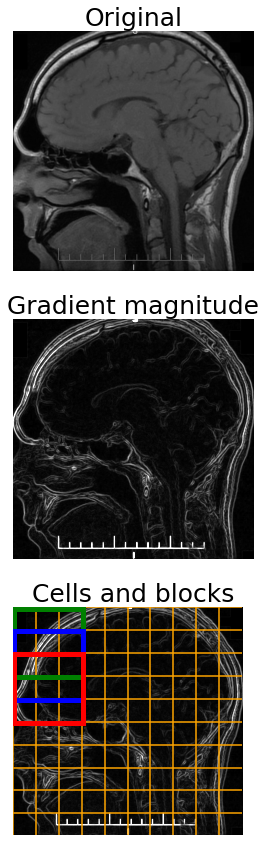
\includegraphics[width=.85\textwidth]{HOG_pt1.png}
        \end{column}
        \pause
        \begin{column}{.8\textwidth}
            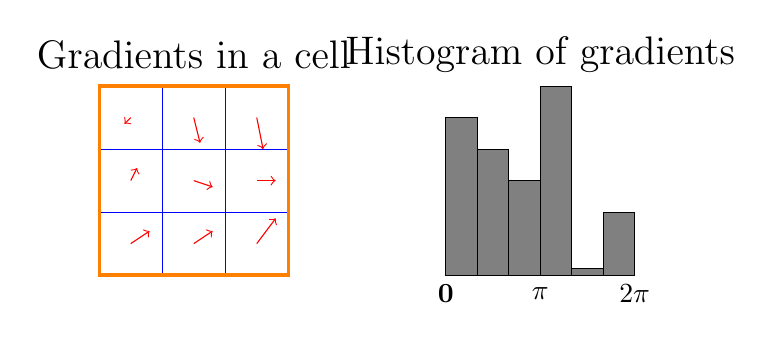
\begin{tikzpicture}[scale=.8]
                \draw [color=blue, step=1, very thin] (0, 0) grid (3, 3);
                \draw [color=orange, very thick] (0, 0) rectangle (3, 3);
                \draw [color=red, ->] (0.5, 0.5) -- (0.8, 0.7);
                \draw [color=red, ->] (0.5, 1.5) -- (0.6, 1.7);
                \draw [color=red, ->] (0.5, 2.5) -- (0.4, 2.4);

                \draw [color=red, ->] (1.5, 0.5) -- (1.8, 0.7);
                \draw [color=red, ->] (1.5, 1.5) -- (1.8, 1.4);
                \draw [color=red, ->] (1.5, 2.5) -- (1.6, 2.1);

                \draw [color=red, ->] (2.5, 0.5) -- (2.8, 0.9);
                \draw [color=red, ->] (2.5, 1.5) -- (2.8, 1.5);
                \draw [color=red, ->] (2.5, 2.5) -- (2.6, 2.0);

                \node at (1.5, 3.5) {\Large Gradients in a cell};

                \node at (7, 3.5) {\Large Histogram of gradients};

                \draw [fill=gray] (5.5, 0) rectangle (6, 2.5);
                \draw [fill=gray] (6, 0) rectangle (6.5, 2);
                \draw [fill=gray] (6.5, 0) rectangle (7, 1.5);
                \draw [fill=gray] (7, 0) rectangle (7.5, 3);
                \draw [fill=gray] (7.5, 0) rectangle (8, 0.1);
                \draw [fill=gray] (8, 0) rectangle (8.5, 1);

                \node at (5.5, -0.3) {\textbf{0}};
                \node at (7, -0.3) {\textbf{$\pi$}};
                \node at (8.5, -0.3) {\textbf{$2\pi$}};

            \end{tikzpicture}
            \pause
            \centering
            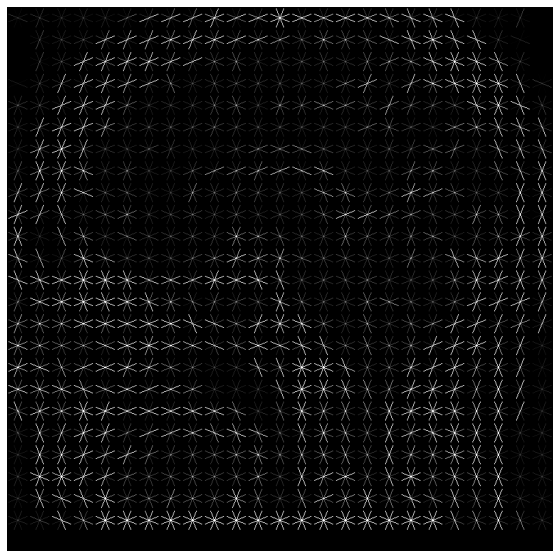
\includegraphics[width=.4\textwidth]{HOG.png}
        \end{column}
    \end{columns}
\end{frame}

\begin{frame}
    {HOG features in Scikit-Image}
    \begin{codebox}
        \texttt{from skimage.feature import hog\\
            from skimage.filters.edges import sobel\\
            from skimage.io import imread\\
            \\
            img = imread('MRI.jpg')\\
            img\_sobel = sobel(img)\\
            \# Because visualize is True, hog returns a tuple of  (feature vector, HOG image)\\
            fd, hog\_image = hog(img\_sobel, orientations=4,\\
            pixels\_per\_cell=(32, 32), cells\_per\_block=(5, 5),\\
            visualize=True)}
    \end{codebox}
\end{frame}

\begin{frame}
{Summary}

\begin{enumerate}
\item Feature extraction is a very important step in image analysis.
\item Features can be fed to machine learning models, or used to detect specific objects in an image.
\item Many other feature detectors exist, and many are implemented in \texttt{skimage.feature} 
\end{enumerate}

\end{frame}
\end{document}

